\section{Ti\-Xml\-Unknown Class Reference}
\label{classTiXmlUnknown}\index{TiXmlUnknown@{TiXmlUnknown}}
Any tag that tiny\-Xml doesn't recognize is saved as an unknown.  


{\tt \#include $<$tinyxml.h$>$}

Inheritance diagram for Ti\-Xml\-Unknown::\begin{figure}[H]
\begin{center}
\leavevmode
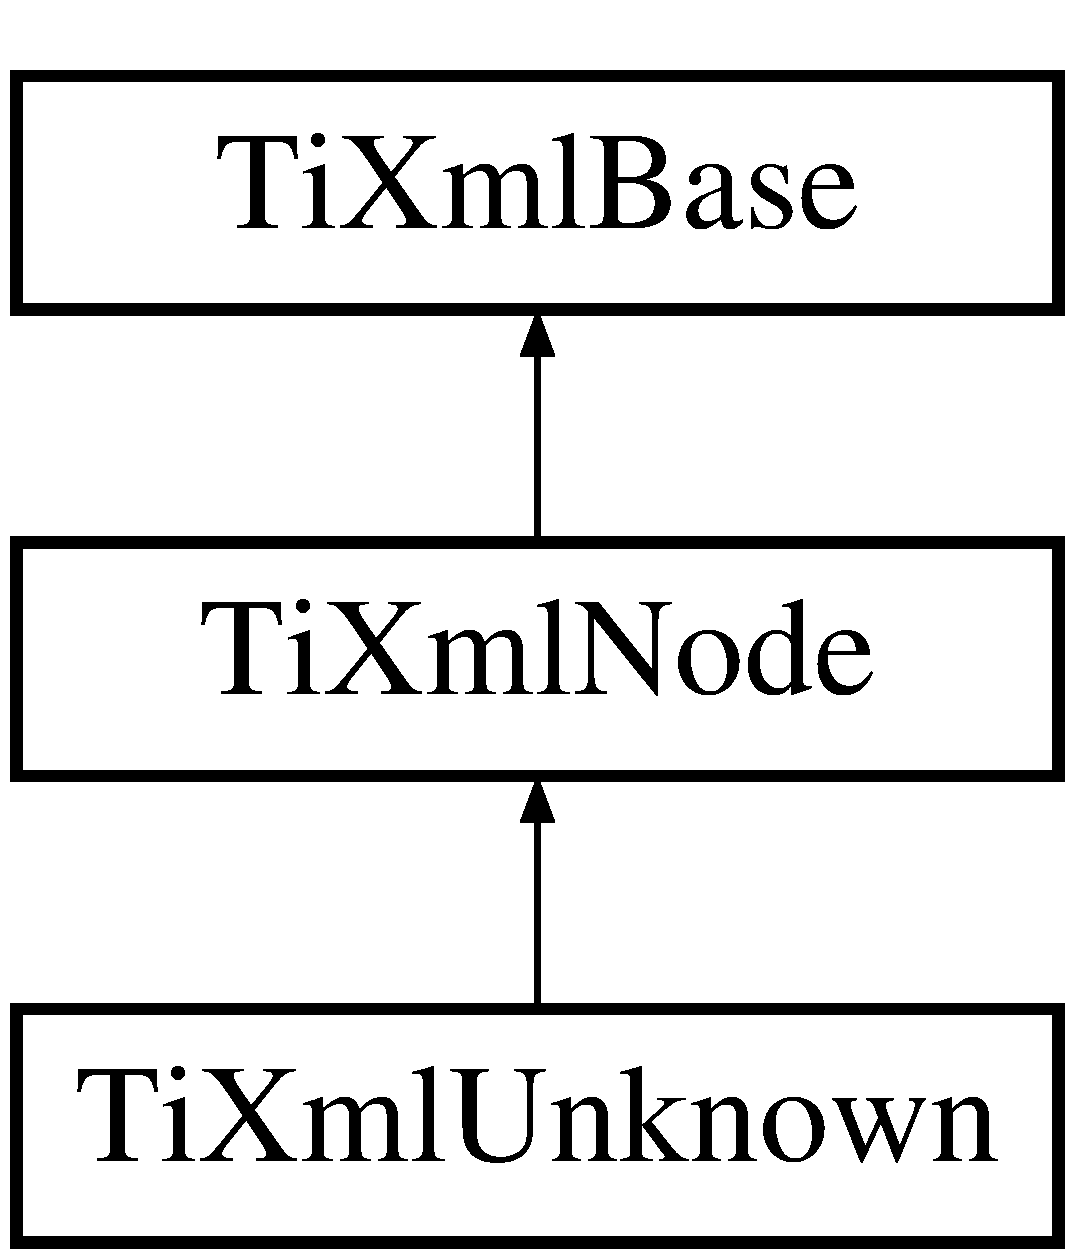
\includegraphics[height=3cm]{classTiXmlUnknown}
\end{center}
\end{figure}
\subsection*{Public Types}
\begin{CompactItemize}
\item 
enum {\bf Node\-Type} \{ \par
{\bf DOCUMENT}, 
{\bf ELEMENT}, 
{\bf COMMENT}, 
{\bf UNKNOWN}, 
\par
{\bf TEXT}, 
{\bf DECLARATION}, 
{\bf TYPECOUNT}
 \}
\begin{CompactList}\small\item\em The types of XML nodes supported by Tiny\-Xml. \item\end{CompactList}\item 
enum \{ \par
{\bf TIXML\_\-NO\_\-ERROR} =  0, 
{\bf TIXML\_\-ERROR}, 
{\bf TIXML\_\-ERROR\_\-OPENING\_\-FILE}, 
{\bf TIXML\_\-ERROR\_\-OUT\_\-OF\_\-MEMORY}, 
\par
{\bf TIXML\_\-ERROR\_\-PARSING\_\-ELEMENT}, 
{\bf TIXML\_\-ERROR\_\-FAILED\_\-TO\_\-READ\_\-ELEMENT\_\-NAME}, 
{\bf TIXML\_\-ERROR\_\-READING\_\-ELEMENT\_\-VALUE}, 
{\bf TIXML\_\-ERROR\_\-READING\_\-ATTRIBUTES}, 
\par
{\bf TIXML\_\-ERROR\_\-PARSING\_\-EMPTY}, 
{\bf TIXML\_\-ERROR\_\-READING\_\-END\_\-TAG}, 
{\bf TIXML\_\-ERROR\_\-PARSING\_\-UNKNOWN}, 
{\bf TIXML\_\-ERROR\_\-PARSING\_\-COMMENT}, 
\par
{\bf TIXML\_\-ERROR\_\-PARSING\_\-DECLARATION}, 
{\bf TIXML\_\-ERROR\_\-DOCUMENT\_\-EMPTY}, 
{\bf TIXML\_\-ERROR\_\-EMBEDDED\_\-NULL}, 
{\bf TIXML\_\-ERROR\_\-PARSING\_\-CDATA}, 
\par
{\bf TIXML\_\-ERROR\_\-STRING\_\-COUNT}
 \}
\end{CompactItemize}
\subsection*{Public Member Functions}
\begin{CompactItemize}
\item 
{\bf Ti\-Xml\-Unknown} (const {\bf Ti\-Xml\-Unknown} \&copy)\label{classTiXmlUnknown_TiXmlUnknowna2}

\item 
void {\bf operator=} (const {\bf Ti\-Xml\-Unknown} \&copy)\label{classTiXmlUnknown_TiXmlUnknowna3}

\item 
virtual {\bf Ti\-Xml\-Node} $\ast$ {\bf Clone} () const\label{classTiXmlUnknown_TiXmlUnknowna4}

\begin{CompactList}\small\item\em Creates a copy of this Unknown and returns it. \item\end{CompactList}\item 
virtual void {\bf Print} (FILE $\ast$cfile, int depth) const\label{classTiXmlUnknown_TiXmlUnknowna5}

\begin{CompactList}\small\item\em Print this Unknown to a FILE stream. \item\end{CompactList}\item 
virtual const char $\ast$ {\bf Parse} (const char $\ast$p, Ti\-Xml\-Parsing\-Data $\ast$data, Ti\-Xml\-Encoding encoding)\label{classTiXmlUnknown_TiXmlUnknowna6}

\item 
const char $\ast$ {\bf Value} () const
\begin{CompactList}\small\item\em The meaning of 'value' changes for the specific type of Ti\-Xml\-Node. \item\end{CompactList}\item 
const std::string \& {\bf Value\-Str} () const
\begin{CompactList}\small\item\em Return {\bf Value()}{\rm (p.\,\pageref{classTiXmlNode_TiXmlUnknowna7})} as a std::string. \item\end{CompactList}\item 
void {\bf Set\-Value} (const char $\ast$\_\-value)
\begin{CompactList}\small\item\em Changes the value of the node. \item\end{CompactList}\item 
void {\bf Set\-Value} (const std::string \&\_\-value)\label{classTiXmlNode_TiXmlUnknowna10}

\begin{CompactList}\small\item\em STL std::string form. \item\end{CompactList}\item 
void {\bf Clear} ()\label{classTiXmlNode_TiXmlUnknowna11}

\begin{CompactList}\small\item\em Delete all the children of this node. Does not affect 'this'. \item\end{CompactList}\item 
{\bf Ti\-Xml\-Node} $\ast$ {\bf Parent} ()\label{classTiXmlNode_TiXmlUnknowna12}

\begin{CompactList}\small\item\em One step up the DOM. \item\end{CompactList}\item 
const {\bf Ti\-Xml\-Node} $\ast$ {\bf Parent} () const\label{classTiXmlNode_TiXmlUnknowna13}

\item 
const {\bf Ti\-Xml\-Node} $\ast$ {\bf First\-Child} () const\label{classTiXmlNode_TiXmlUnknowna14}

\begin{CompactList}\small\item\em The first child of this node. Will be null if there are no children. \item\end{CompactList}\item 
{\bf Ti\-Xml\-Node} $\ast$ {\bf First\-Child} ()\label{classTiXmlNode_TiXmlUnknowna15}

\item 
const {\bf Ti\-Xml\-Node} $\ast$ {\bf First\-Child} (const char $\ast$value) const\label{classTiXmlNode_TiXmlUnknowna16}

\begin{CompactList}\small\item\em The first child of this node with the matching 'value'. Will be null if none found. \item\end{CompactList}\item 
{\bf Ti\-Xml\-Node} $\ast$ {\bf First\-Child} (const char $\ast$value)\label{classTiXmlNode_TiXmlUnknowna17}

\begin{CompactList}\small\item\em The first child of this node with the matching 'value'. Will be null if none found. \item\end{CompactList}\item 
const {\bf Ti\-Xml\-Node} $\ast$ {\bf First\-Child} (const std::string \&\_\-value) const\label{classTiXmlNode_TiXmlUnknowna18}

\begin{CompactList}\small\item\em STL std::string form. \item\end{CompactList}\item 
{\bf Ti\-Xml\-Node} $\ast$ {\bf First\-Child} (const std::string \&\_\-value)\label{classTiXmlNode_TiXmlUnknowna19}

\begin{CompactList}\small\item\em STL std::string form. \item\end{CompactList}\item 
const {\bf Ti\-Xml\-Node} $\ast$ {\bf Last\-Child} () const\label{classTiXmlNode_TiXmlUnknowna20}

\item 
{\bf Ti\-Xml\-Node} $\ast$ {\bf Last\-Child} ()\label{classTiXmlNode_TiXmlUnknowna21}

\begin{CompactList}\small\item\em The last child of this node. Will be null if there are no children. \item\end{CompactList}\item 
const {\bf Ti\-Xml\-Node} $\ast$ {\bf Last\-Child} (const char $\ast$value) const\label{classTiXmlNode_TiXmlUnknowna22}

\item 
{\bf Ti\-Xml\-Node} $\ast$ {\bf Last\-Child} (const char $\ast$value)\label{classTiXmlNode_TiXmlUnknowna23}

\begin{CompactList}\small\item\em The last child of this node matching 'value'. Will be null if there are no children. \item\end{CompactList}\item 
const {\bf Ti\-Xml\-Node} $\ast$ {\bf Last\-Child} (const std::string \&\_\-value) const\label{classTiXmlNode_TiXmlUnknowna24}

\begin{CompactList}\small\item\em STL std::string form. \item\end{CompactList}\item 
{\bf Ti\-Xml\-Node} $\ast$ {\bf Last\-Child} (const std::string \&\_\-value)\label{classTiXmlNode_TiXmlUnknowna25}

\begin{CompactList}\small\item\em STL std::string form. \item\end{CompactList}\item 
const {\bf Ti\-Xml\-Node} $\ast$ {\bf Iterate\-Children} (const {\bf Ti\-Xml\-Node} $\ast$previous) const
\begin{CompactList}\small\item\em An alternate way to walk the children of a node. \item\end{CompactList}\item 
{\bf Ti\-Xml\-Node} $\ast$ {\bf Iterate\-Children} ({\bf Ti\-Xml\-Node} $\ast$previous)\label{classTiXmlNode_TiXmlUnknowna27}

\item 
const {\bf Ti\-Xml\-Node} $\ast$ {\bf Iterate\-Children} (const char $\ast$value, const {\bf Ti\-Xml\-Node} $\ast$previous) const\label{classTiXmlNode_TiXmlUnknowna28}

\begin{CompactList}\small\item\em This flavor of Iterate\-Children searches for children with a particular 'value'. \item\end{CompactList}\item 
{\bf Ti\-Xml\-Node} $\ast$ {\bf Iterate\-Children} (const char $\ast$value, {\bf Ti\-Xml\-Node} $\ast$previous)\label{classTiXmlNode_TiXmlUnknowna29}

\item 
const {\bf Ti\-Xml\-Node} $\ast$ {\bf Iterate\-Children} (const std::string \&\_\-value, const {\bf Ti\-Xml\-Node} $\ast$previous) const\label{classTiXmlNode_TiXmlUnknowna30}

\begin{CompactList}\small\item\em STL std::string form. \item\end{CompactList}\item 
{\bf Ti\-Xml\-Node} $\ast$ {\bf Iterate\-Children} (const std::string \&\_\-value, {\bf Ti\-Xml\-Node} $\ast$previous)\label{classTiXmlNode_TiXmlUnknowna31}

\begin{CompactList}\small\item\em STL std::string form. \item\end{CompactList}\item 
{\bf Ti\-Xml\-Node} $\ast$ {\bf Insert\-End\-Child} (const {\bf Ti\-Xml\-Node} \&add\-This)
\begin{CompactList}\small\item\em Add a new node related to this. \item\end{CompactList}\item 
{\bf Ti\-Xml\-Node} $\ast$ {\bf Link\-End\-Child} ({\bf Ti\-Xml\-Node} $\ast$add\-This)
\begin{CompactList}\small\item\em Add a new node related to this. \item\end{CompactList}\item 
{\bf Ti\-Xml\-Node} $\ast$ {\bf Insert\-Before\-Child} ({\bf Ti\-Xml\-Node} $\ast$before\-This, const {\bf Ti\-Xml\-Node} \&add\-This)
\begin{CompactList}\small\item\em Add a new node related to this. \item\end{CompactList}\item 
{\bf Ti\-Xml\-Node} $\ast$ {\bf Insert\-After\-Child} ({\bf Ti\-Xml\-Node} $\ast$after\-This, const {\bf Ti\-Xml\-Node} \&add\-This)
\begin{CompactList}\small\item\em Add a new node related to this. \item\end{CompactList}\item 
{\bf Ti\-Xml\-Node} $\ast$ {\bf Replace\-Child} ({\bf Ti\-Xml\-Node} $\ast$replace\-This, const {\bf Ti\-Xml\-Node} \&with\-This)
\begin{CompactList}\small\item\em Replace a child of this node. \item\end{CompactList}\item 
bool {\bf Remove\-Child} ({\bf Ti\-Xml\-Node} $\ast$remove\-This)\label{classTiXmlNode_TiXmlUnknowna37}

\begin{CompactList}\small\item\em Delete a child of this node. \item\end{CompactList}\item 
const {\bf Ti\-Xml\-Node} $\ast$ {\bf Previous\-Sibling} () const\label{classTiXmlNode_TiXmlUnknowna38}

\begin{CompactList}\small\item\em Navigate to a sibling node. \item\end{CompactList}\item 
{\bf Ti\-Xml\-Node} $\ast$ {\bf Previous\-Sibling} ()\label{classTiXmlNode_TiXmlUnknowna39}

\item 
const {\bf Ti\-Xml\-Node} $\ast$ {\bf Previous\-Sibling} (const char $\ast$) const\label{classTiXmlNode_TiXmlUnknowna40}

\begin{CompactList}\small\item\em Navigate to a sibling node. \item\end{CompactList}\item 
{\bf Ti\-Xml\-Node} $\ast$ {\bf Previous\-Sibling} (const char $\ast$)\label{classTiXmlNode_TiXmlUnknowna41}

\item 
const {\bf Ti\-Xml\-Node} $\ast$ {\bf Previous\-Sibling} (const std::string \&\_\-value) const\label{classTiXmlNode_TiXmlUnknowna42}

\begin{CompactList}\small\item\em STL std::string form. \item\end{CompactList}\item 
{\bf Ti\-Xml\-Node} $\ast$ {\bf Previous\-Sibling} (const std::string \&\_\-value)\label{classTiXmlNode_TiXmlUnknowna43}

\begin{CompactList}\small\item\em STL std::string form. \item\end{CompactList}\item 
const {\bf Ti\-Xml\-Node} $\ast$ {\bf Next\-Sibling} (const std::string \&\_\-value) const\label{classTiXmlNode_TiXmlUnknowna44}

\begin{CompactList}\small\item\em STL std::string form. \item\end{CompactList}\item 
{\bf Ti\-Xml\-Node} $\ast$ {\bf Next\-Sibling} (const std::string \&\_\-value)\label{classTiXmlNode_TiXmlUnknowna45}

\begin{CompactList}\small\item\em STL std::string form. \item\end{CompactList}\item 
const {\bf Ti\-Xml\-Node} $\ast$ {\bf Next\-Sibling} () const\label{classTiXmlNode_TiXmlUnknowna46}

\begin{CompactList}\small\item\em Navigate to a sibling node. \item\end{CompactList}\item 
{\bf Ti\-Xml\-Node} $\ast$ {\bf Next\-Sibling} ()\label{classTiXmlNode_TiXmlUnknowna47}

\item 
const {\bf Ti\-Xml\-Node} $\ast$ {\bf Next\-Sibling} (const char $\ast$) const\label{classTiXmlNode_TiXmlUnknowna48}

\begin{CompactList}\small\item\em Navigate to a sibling node with the given 'value'. \item\end{CompactList}\item 
{\bf Ti\-Xml\-Node} $\ast$ {\bf Next\-Sibling} (const char $\ast$)\label{classTiXmlNode_TiXmlUnknowna49}

\item 
const {\bf Ti\-Xml\-Element} $\ast$ {\bf Next\-Sibling\-Element} () const
\begin{CompactList}\small\item\em Convenience function to get through elements. \item\end{CompactList}\item 
{\bf Ti\-Xml\-Element} $\ast$ {\bf Next\-Sibling\-Element} ()\label{classTiXmlNode_TiXmlUnknowna51}

\item 
const {\bf Ti\-Xml\-Element} $\ast$ {\bf Next\-Sibling\-Element} (const char $\ast$) const
\begin{CompactList}\small\item\em Convenience function to get through elements. \item\end{CompactList}\item 
{\bf Ti\-Xml\-Element} $\ast$ {\bf Next\-Sibling\-Element} (const char $\ast$)\label{classTiXmlNode_TiXmlUnknowna53}

\item 
const {\bf Ti\-Xml\-Element} $\ast$ {\bf Next\-Sibling\-Element} (const std::string \&\_\-value) const\label{classTiXmlNode_TiXmlUnknowna54}

\begin{CompactList}\small\item\em STL std::string form. \item\end{CompactList}\item 
{\bf Ti\-Xml\-Element} $\ast$ {\bf Next\-Sibling\-Element} (const std::string \&\_\-value)\label{classTiXmlNode_TiXmlUnknowna55}

\begin{CompactList}\small\item\em STL std::string form. \item\end{CompactList}\item 
const {\bf Ti\-Xml\-Element} $\ast$ {\bf First\-Child\-Element} () const\label{classTiXmlNode_TiXmlUnknowna56}

\begin{CompactList}\small\item\em Convenience function to get through elements. \item\end{CompactList}\item 
{\bf Ti\-Xml\-Element} $\ast$ {\bf First\-Child\-Element} ()\label{classTiXmlNode_TiXmlUnknowna57}

\item 
const {\bf Ti\-Xml\-Element} $\ast$ {\bf First\-Child\-Element} (const char $\ast$value) const\label{classTiXmlNode_TiXmlUnknowna58}

\begin{CompactList}\small\item\em Convenience function to get through elements. \item\end{CompactList}\item 
{\bf Ti\-Xml\-Element} $\ast$ {\bf First\-Child\-Element} (const char $\ast$value)\label{classTiXmlNode_TiXmlUnknowna59}

\item 
const {\bf Ti\-Xml\-Element} $\ast$ {\bf First\-Child\-Element} (const std::string \&\_\-value) const\label{classTiXmlNode_TiXmlUnknowna60}

\begin{CompactList}\small\item\em STL std::string form. \item\end{CompactList}\item 
{\bf Ti\-Xml\-Element} $\ast$ {\bf First\-Child\-Element} (const std::string \&\_\-value)\label{classTiXmlNode_TiXmlUnknowna61}

\begin{CompactList}\small\item\em STL std::string form. \item\end{CompactList}\item 
int {\bf Type} () const
\begin{CompactList}\small\item\em Query the type (as an enumerated value, above) of this node. \item\end{CompactList}\item 
const {\bf Ti\-Xml\-Document} $\ast$ {\bf Get\-Document} () const
\begin{CompactList}\small\item\em Return a pointer to the Document this node lives in. \item\end{CompactList}\item 
{\bf Ti\-Xml\-Document} $\ast$ {\bf Get\-Document} ()\label{classTiXmlNode_TiXmlUnknowna64}

\item 
bool {\bf No\-Children} () const\label{classTiXmlNode_TiXmlUnknowna65}

\begin{CompactList}\small\item\em Returns true if this node has no children. \item\end{CompactList}\item 
const {\bf Ti\-Xml\-Document} $\ast$ {\bf To\-Document} () const\label{classTiXmlNode_TiXmlUnknowna66}

\begin{CompactList}\small\item\em Cast to a more defined type. Will return null not of the requested type. \item\end{CompactList}\item 
{\bf Ti\-Xml\-Document} $\ast$ {\bf To\-Document} ()\label{classTiXmlNode_TiXmlUnknowna67}

\begin{CompactList}\small\item\em Cast to a more defined type. Will return null not of the requested type. \item\end{CompactList}\item 
const {\bf Ti\-Xml\-Element} $\ast$ {\bf To\-Element} () const\label{classTiXmlNode_TiXmlUnknowna68}

\begin{CompactList}\small\item\em Cast to a more defined type. Will return null not of the requested type. \item\end{CompactList}\item 
{\bf Ti\-Xml\-Element} $\ast$ {\bf To\-Element} ()\label{classTiXmlNode_TiXmlUnknowna69}

\begin{CompactList}\small\item\em Cast to a more defined type. Will return null not of the requested type. \item\end{CompactList}\item 
const {\bf Ti\-Xml\-Comment} $\ast$ {\bf To\-Comment} () const\label{classTiXmlNode_TiXmlUnknowna70}

\begin{CompactList}\small\item\em Cast to a more defined type. Will return null not of the requested type. \item\end{CompactList}\item 
{\bf Ti\-Xml\-Comment} $\ast$ {\bf To\-Comment} ()\label{classTiXmlNode_TiXmlUnknowna71}

\begin{CompactList}\small\item\em Cast to a more defined type. Will return null not of the requested type. \item\end{CompactList}\item 
const {\bf Ti\-Xml\-Unknown} $\ast$ {\bf To\-Unknown} () const\label{classTiXmlNode_TiXmlUnknowna72}

\begin{CompactList}\small\item\em Cast to a more defined type. Will return null not of the requested type. \item\end{CompactList}\item 
{\bf Ti\-Xml\-Unknown} $\ast$ {\bf To\-Unknown} ()\label{classTiXmlNode_TiXmlUnknowna73}

\begin{CompactList}\small\item\em Cast to a more defined type. Will return null not of the requested type. \item\end{CompactList}\item 
const {\bf Ti\-Xml\-Text} $\ast$ {\bf To\-Text} () const\label{classTiXmlNode_TiXmlUnknowna74}

\begin{CompactList}\small\item\em Cast to a more defined type. Will return null not of the requested type. \item\end{CompactList}\item 
{\bf Ti\-Xml\-Text} $\ast$ {\bf To\-Text} ()\label{classTiXmlNode_TiXmlUnknowna75}

\begin{CompactList}\small\item\em Cast to a more defined type. Will return null not of the requested type. \item\end{CompactList}\item 
const {\bf Ti\-Xml\-Declaration} $\ast$ {\bf To\-Declaration} () const\label{classTiXmlNode_TiXmlUnknowna76}

\begin{CompactList}\small\item\em Cast to a more defined type. Will return null not of the requested type. \item\end{CompactList}\item 
{\bf Ti\-Xml\-Declaration} $\ast$ {\bf To\-Declaration} ()\label{classTiXmlNode_TiXmlUnknowna77}

\begin{CompactList}\small\item\em Cast to a more defined type. Will return null not of the requested type. \item\end{CompactList}\item 
int {\bf Row} () const
\begin{CompactList}\small\item\em Return the position, in the original source file, of this node or attribute. \item\end{CompactList}\item 
int {\bf Column} () const\label{classTiXmlBase_TiXmlUnknowna79}

\begin{CompactList}\small\item\em See {\bf Row()}{\rm (p.\,\pageref{classTiXmlBase_TiXmlUnknowna78})}. \item\end{CompactList}\item 
void {\bf Set\-User\-Data} (void $\ast$user)\label{classTiXmlBase_TiXmlUnknowna80}

\item 
void $\ast$ {\bf Get\-User\-Data} ()\label{classTiXmlBase_TiXmlUnknowna81}

\end{CompactItemize}
\subsection*{Static Public Member Functions}
\begin{CompactItemize}
\item 
void {\bf Set\-Condense\-White\-Space} (bool condense)
\begin{CompactList}\small\item\em The world does not agree on whether white space should be kept or not. \item\end{CompactList}\item 
bool {\bf Is\-White\-Space\-Condensed} ()\label{classTiXmlBase_TiXmlUnknowne1}

\begin{CompactList}\small\item\em Return the current white space setting. \item\end{CompactList}\end{CompactItemize}
\subsection*{Static Public Attributes}
\begin{CompactItemize}
\item 
const int {\bf utf8Byte\-Table} [256]
\end{CompactItemize}
\subsection*{Protected Member Functions}
\begin{CompactItemize}
\item 
void {\bf Copy\-To} ({\bf Ti\-Xml\-Unknown} $\ast$target) const\label{classTiXmlUnknown_TiXmlUnknownb0}

\item 
virtual void {\bf Stream\-In} (TIXML\_\-ISTREAM $\ast$in, TIXML\_\-STRING $\ast$tag)\label{classTiXmlUnknown_TiXmlUnknownb1}

\item 
virtual void {\bf Stream\-Out} (TIXML\_\-OSTREAM $\ast$out) const\label{classTiXmlUnknown_TiXmlUnknownb2}

\item 
void {\bf Copy\-To} ({\bf Ti\-Xml\-Node} $\ast$target) const\label{classTiXmlNode_TiXmlUnknownb3}

\item 
{\bf Ti\-Xml\-Node} $\ast$ {\bf Identify} (const char $\ast$start, Ti\-Xml\-Encoding encoding)\label{classTiXmlNode_TiXmlUnknownb4}

\end{CompactItemize}
\subsection*{Static Protected Member Functions}
\begin{CompactItemize}
\item 
const char $\ast$ {\bf Skip\-White\-Space} (const char $\ast$, Ti\-Xml\-Encoding encoding)\label{classTiXmlBase_TiXmlUnknownf0}

\item 
bool {\bf Is\-White\-Space} (char c)\label{classTiXmlBase_TiXmlUnknownf1}

\item 
bool {\bf Stream\-White\-Space} (TIXML\_\-ISTREAM $\ast$in, TIXML\_\-STRING $\ast$tag)\label{classTiXmlBase_TiXmlUnknownf2}

\item 
bool {\bf Stream\-To} (TIXML\_\-ISTREAM $\ast$in, int character, TIXML\_\-STRING $\ast$tag)\label{classTiXmlBase_TiXmlUnknownf3}

\item 
const char $\ast$ {\bf Read\-Name} (const char $\ast$p, TIXML\_\-STRING $\ast$name, Ti\-Xml\-Encoding encoding)\label{classTiXmlBase_TiXmlUnknownf4}

\item 
const char $\ast$ {\bf Read\-Text} (const char $\ast$in, TIXML\_\-STRING $\ast$text, bool ignore\-White\-Space, const char $\ast$end\-Tag, bool ignore\-Case, Ti\-Xml\-Encoding encoding)\label{classTiXmlBase_TiXmlUnknownf5}

\item 
const char $\ast$ {\bf Get\-Entity} (const char $\ast$in, char $\ast$value, int $\ast$length, Ti\-Xml\-Encoding encoding)\label{classTiXmlBase_TiXmlUnknownf6}

\item 
const char $\ast$ {\bf Get\-Char} (const char $\ast$p, char $\ast$\_\-value, int $\ast$length, Ti\-Xml\-Encoding encoding)\label{classTiXmlBase_TiXmlUnknownf7}

\item 
void {\bf Put\-String} (const TIXML\_\-STRING \&str, TIXML\_\-OSTREAM $\ast$out)\label{classTiXmlBase_TiXmlUnknownf8}

\item 
void {\bf Put\-String} (const TIXML\_\-STRING \&str, TIXML\_\-STRING $\ast$out)\label{classTiXmlBase_TiXmlUnknownf9}

\item 
bool {\bf String\-Equal} (const char $\ast$p, const char $\ast$end\-Tag, bool ignore\-Case, Ti\-Xml\-Encoding encoding)\label{classTiXmlBase_TiXmlUnknownf10}

\item 
int {\bf Is\-Alpha} (unsigned char any\-Byte, Ti\-Xml\-Encoding encoding)\label{classTiXmlBase_TiXmlUnknownf11}

\item 
int {\bf Is\-Alpha\-Num} (unsigned char any\-Byte, Ti\-Xml\-Encoding encoding)\label{classTiXmlBase_TiXmlUnknownf12}

\item 
int {\bf To\-Lower} (int v, Ti\-Xml\-Encoding encoding)\label{classTiXmlBase_TiXmlUnknownf13}

\item 
void {\bf Convert\-UTF32To\-UTF8} (unsigned long input, char $\ast$output, int $\ast$length)\label{classTiXmlBase_TiXmlUnknownf14}

\end{CompactItemize}
\subsection*{Protected Attributes}
\begin{CompactItemize}
\item 
{\bf Ti\-Xml\-Node} $\ast$ {\bf parent}\label{classTiXmlNode_TiXmlUnknownp0}

\item 
{\bf Node\-Type} {\bf type}\label{classTiXmlNode_TiXmlUnknownp1}

\item 
{\bf Ti\-Xml\-Node} $\ast$ {\bf first\-Child}\label{classTiXmlNode_TiXmlUnknownp2}

\item 
{\bf Ti\-Xml\-Node} $\ast$ {\bf last\-Child}\label{classTiXmlNode_TiXmlUnknownp3}

\item 
TIXML\_\-STRING {\bf value}\label{classTiXmlNode_TiXmlUnknownp4}

\item 
{\bf Ti\-Xml\-Node} $\ast$ {\bf prev}\label{classTiXmlNode_TiXmlUnknownp5}

\item 
{\bf Ti\-Xml\-Node} $\ast$ {\bf next}\label{classTiXmlNode_TiXmlUnknownp6}

\item 
Ti\-Xml\-Cursor {\bf location}\label{classTiXmlBase_TiXmlUnknownp7}

\item 
void $\ast$ {\bf user\-Data}\label{classTiXmlBase_TiXmlUnknownp8}

\begin{CompactList}\small\item\em Field containing a generic user pointer. \item\end{CompactList}\end{CompactItemize}
\subsection*{Static Protected Attributes}
\begin{CompactItemize}
\item 
const char $\ast$ {\bf error\-String} [TIXML\_\-ERROR\_\-STRING\_\-COUNT]
\end{CompactItemize}
\subsection*{Friends}
\begin{CompactItemize}
\item 
std::istream \& {\bf operator$>$$>$} (std::istream \&in, {\bf Ti\-Xml\-Node} \&base)
\begin{CompactList}\small\item\em An input stream operator, for every class. \item\end{CompactList}\item 
std::ostream \& {\bf operator$<$$<$} (std::ostream \&out, const {\bf Ti\-Xml\-Node} \&base)
\begin{CompactList}\small\item\em An output stream operator, for every class. \item\end{CompactList}\item 
std::string \& {\bf operator$<$$<$} (std::string \&out, const {\bf Ti\-Xml\-Node} \&base)\label{classTiXmlNode_TiXmlUnknownn2}

\begin{CompactList}\small\item\em Appends the XML node or attribute to a std::string. \item\end{CompactList}\end{CompactItemize}


\subsection{Detailed Description}
Any tag that tiny\-Xml doesn't recognize is saved as an unknown. 

It is a tag of text, but should not be modified. It will be written back to the XML, unchanged, when the file is saved.

DTD tags get thrown into Ti\-Xml\-Unknowns. 



\subsection{Member Enumeration Documentation}
\index{TiXmlUnknown@{Ti\-Xml\-Unknown}!NodeType@{NodeType}}
\index{NodeType@{NodeType}!TiXmlUnknown@{Ti\-Xml\-Unknown}}
\subsubsection{\setlength{\rightskip}{0pt plus 5cm}enum {\bf Ti\-Xml\-Node::Node\-Type}\hspace{0.3cm}{\tt  [inherited]}}\label{classTiXmlNode_TiXmlUnknownw7}


The types of XML nodes supported by Tiny\-Xml. 

(All the unsupported types are picked up by UNKNOWN.)

\subsection{Member Function Documentation}
\index{TiXmlUnknown@{Ti\-Xml\-Unknown}!GetDocument@{GetDocument}}
\index{GetDocument@{GetDocument}!TiXmlUnknown@{Ti\-Xml\-Unknown}}
\subsubsection{\setlength{\rightskip}{0pt plus 5cm}const {\bf Ti\-Xml\-Document} $\ast$ Ti\-Xml\-Node::Get\-Document () const\hspace{0.3cm}{\tt  [inherited]}}\label{classTiXmlNode_TiXmlUnknowna63}


Return a pointer to the Document this node lives in. 

Returns null if not in a document.\index{TiXmlUnknown@{Ti\-Xml\-Unknown}!InsertAfterChild@{InsertAfterChild}}
\index{InsertAfterChild@{InsertAfterChild}!TiXmlUnknown@{Ti\-Xml\-Unknown}}
\subsubsection{\setlength{\rightskip}{0pt plus 5cm}{\bf Ti\-Xml\-Node} $\ast$ Ti\-Xml\-Node::Insert\-After\-Child ({\bf Ti\-Xml\-Node} $\ast$ {\em after\-This}, const {\bf Ti\-Xml\-Node} \& {\em add\-This})\hspace{0.3cm}{\tt  [inherited]}}\label{classTiXmlNode_TiXmlUnknowna35}


Add a new node related to this. 

Adds a child after the specified child. Returns a pointer to the new object or NULL if an error occured.\index{TiXmlUnknown@{Ti\-Xml\-Unknown}!InsertBeforeChild@{InsertBeforeChild}}
\index{InsertBeforeChild@{InsertBeforeChild}!TiXmlUnknown@{Ti\-Xml\-Unknown}}
\subsubsection{\setlength{\rightskip}{0pt plus 5cm}{\bf Ti\-Xml\-Node} $\ast$ Ti\-Xml\-Node::Insert\-Before\-Child ({\bf Ti\-Xml\-Node} $\ast$ {\em before\-This}, const {\bf Ti\-Xml\-Node} \& {\em add\-This})\hspace{0.3cm}{\tt  [inherited]}}\label{classTiXmlNode_TiXmlUnknowna34}


Add a new node related to this. 

Adds a child before the specified child. Returns a pointer to the new object or NULL if an error occured.\index{TiXmlUnknown@{Ti\-Xml\-Unknown}!InsertEndChild@{InsertEndChild}}
\index{InsertEndChild@{InsertEndChild}!TiXmlUnknown@{Ti\-Xml\-Unknown}}
\subsubsection{\setlength{\rightskip}{0pt plus 5cm}{\bf Ti\-Xml\-Node} $\ast$ Ti\-Xml\-Node::Insert\-End\-Child (const {\bf Ti\-Xml\-Node} \& {\em add\-This})\hspace{0.3cm}{\tt  [inherited]}}\label{classTiXmlNode_TiXmlUnknowna32}


Add a new node related to this. 

Adds a child past the Last\-Child. Returns a pointer to the new object or NULL if an error occured.\index{TiXmlUnknown@{Ti\-Xml\-Unknown}!IterateChildren@{IterateChildren}}
\index{IterateChildren@{IterateChildren}!TiXmlUnknown@{Ti\-Xml\-Unknown}}
\subsubsection{\setlength{\rightskip}{0pt plus 5cm}const {\bf Ti\-Xml\-Node} $\ast$ Ti\-Xml\-Node::Iterate\-Children (const {\bf Ti\-Xml\-Node} $\ast$ {\em previous}) const\hspace{0.3cm}{\tt  [inherited]}}\label{classTiXmlNode_TiXmlUnknowna26}


An alternate way to walk the children of a node. 

One way to iterate over nodes is: 

\footnotesize\begin{verbatim}
			for( child = parent->FirstChild(); child; child = child->NextSibling() )
		\end{verbatim}
\normalsize


Iterate\-Children does the same thing with the syntax: 

\footnotesize\begin{verbatim}
			child = 0;
			while( child = parent->IterateChildren( child ) )
		\end{verbatim}
\normalsize


Iterate\-Children takes the previous child as input and finds the next one. If the previous child is null, it returns the first. Iterate\-Children will return null when done.\index{TiXmlUnknown@{Ti\-Xml\-Unknown}!LinkEndChild@{LinkEndChild}}
\index{LinkEndChild@{LinkEndChild}!TiXmlUnknown@{Ti\-Xml\-Unknown}}
\subsubsection{\setlength{\rightskip}{0pt plus 5cm}{\bf Ti\-Xml\-Node} $\ast$ Ti\-Xml\-Node::Link\-End\-Child ({\bf Ti\-Xml\-Node} $\ast$ {\em add\-This})\hspace{0.3cm}{\tt  [inherited]}}\label{classTiXmlNode_TiXmlUnknowna33}


Add a new node related to this. 

Adds a child past the Last\-Child.

NOTE: the node to be added is passed by pointer, and will be henceforth owned (and deleted) by tiny\-Xml. This method is efficient and avoids an extra copy, but should be used with care as it uses a different memory model than the other insert functions.

\begin{Desc}
\item[See also:]{\bf Insert\-End\-Child}{\rm (p.\,\pageref{classTiXmlNode_TiXmlUnknowna32})}\end{Desc}
\index{TiXmlUnknown@{Ti\-Xml\-Unknown}!NextSiblingElement@{NextSiblingElement}}
\index{NextSiblingElement@{NextSiblingElement}!TiXmlUnknown@{Ti\-Xml\-Unknown}}
\subsubsection{\setlength{\rightskip}{0pt plus 5cm}const {\bf Ti\-Xml\-Element} $\ast$ Ti\-Xml\-Node::Next\-Sibling\-Element (const char $\ast$) const\hspace{0.3cm}{\tt  [inherited]}}\label{classTiXmlNode_TiXmlUnknowna52}


Convenience function to get through elements. 

Calls Next\-Sibling and To\-Element. Will skip all non-Element nodes. Returns 0 if there is not another element.\index{TiXmlUnknown@{Ti\-Xml\-Unknown}!NextSiblingElement@{NextSiblingElement}}
\index{NextSiblingElement@{NextSiblingElement}!TiXmlUnknown@{Ti\-Xml\-Unknown}}
\subsubsection{\setlength{\rightskip}{0pt plus 5cm}const {\bf Ti\-Xml\-Element} $\ast$ Ti\-Xml\-Node::Next\-Sibling\-Element () const\hspace{0.3cm}{\tt  [inherited]}}\label{classTiXmlNode_TiXmlUnknowna50}


Convenience function to get through elements. 

Calls Next\-Sibling and To\-Element. Will skip all non-Element nodes. Returns 0 if there is not another element.\index{TiXmlUnknown@{Ti\-Xml\-Unknown}!ReplaceChild@{ReplaceChild}}
\index{ReplaceChild@{ReplaceChild}!TiXmlUnknown@{Ti\-Xml\-Unknown}}
\subsubsection{\setlength{\rightskip}{0pt plus 5cm}{\bf Ti\-Xml\-Node} $\ast$ Ti\-Xml\-Node::Replace\-Child ({\bf Ti\-Xml\-Node} $\ast$ {\em replace\-This}, const {\bf Ti\-Xml\-Node} \& {\em with\-This})\hspace{0.3cm}{\tt  [inherited]}}\label{classTiXmlNode_TiXmlUnknowna36}


Replace a child of this node. 

Returns a pointer to the new object or NULL if an error occured.\index{TiXmlUnknown@{Ti\-Xml\-Unknown}!Row@{Row}}
\index{Row@{Row}!TiXmlUnknown@{Ti\-Xml\-Unknown}}
\subsubsection{\setlength{\rightskip}{0pt plus 5cm}int Ti\-Xml\-Base::Row () const\hspace{0.3cm}{\tt  [inline, inherited]}}\label{classTiXmlBase_TiXmlUnknowna78}


Return the position, in the original source file, of this node or attribute. 

The row and column are 1-based. (That is the first row and first column is 1,1). If the returns values are 0 or less, then the parser does not have a row and column value.

Generally, the row and column value will be set when the Ti\-Xml\-Document::Load(), {\bf Ti\-Xml\-Document::Load\-File()}{\rm (p.\,\pageref{classTiXmlDocument_TiXmlDocumenta6})}, or any Ti\-Xml\-Node::Parse() is called. It will NOT be set when the DOM was created from operator$>$$>$.

The values reflect the initial load. Once the DOM is modified programmatically (by adding or changing nodes and attributes) the new values will NOT update to reflect changes in the document.

There is a minor performance cost to computing the row and column. Computation can be disabled if {\bf Ti\-Xml\-Document::Set\-Tab\-Size()}{\rm (p.\,\pageref{classTiXmlDocument_TiXmlDocumenta20})} is called with 0 as the value.

\begin{Desc}
\item[See also:]{\bf Ti\-Xml\-Document::Set\-Tab\-Size()}{\rm (p.\,\pageref{classTiXmlDocument_TiXmlDocumenta20})}\end{Desc}
\index{TiXmlUnknown@{Ti\-Xml\-Unknown}!SetCondenseWhiteSpace@{SetCondenseWhiteSpace}}
\index{SetCondenseWhiteSpace@{SetCondenseWhiteSpace}!TiXmlUnknown@{Ti\-Xml\-Unknown}}
\subsubsection{\setlength{\rightskip}{0pt plus 5cm}void Ti\-Xml\-Base::Set\-Condense\-White\-Space (bool {\em condense})\hspace{0.3cm}{\tt  [inline, static, inherited]}}\label{classTiXmlBase_TiXmlUnknowne0}


The world does not agree on whether white space should be kept or not. 

In order to make everyone happy, these global, static functions are provided to set whether or not Tiny\-Xml will condense all white space into a single space or not. The default is to condense. Note changing this values is not thread safe.\index{TiXmlUnknown@{Ti\-Xml\-Unknown}!SetValue@{SetValue}}
\index{SetValue@{SetValue}!TiXmlUnknown@{Ti\-Xml\-Unknown}}
\subsubsection{\setlength{\rightskip}{0pt plus 5cm}void Ti\-Xml\-Node::Set\-Value (const char $\ast$ {\em \_\-value})\hspace{0.3cm}{\tt  [inline, inherited]}}\label{classTiXmlNode_TiXmlUnknowna9}


Changes the value of the node. 

Defined as: 

\footnotesize\begin{verbatim}
		Document:	filename of the xml file
		Element:	name of the element
		Comment:	the comment text
		Unknown:	the tag contents
		Text:		the text string
		\end{verbatim}
\normalsize
\index{TiXmlUnknown@{Ti\-Xml\-Unknown}!Type@{Type}}
\index{Type@{Type}!TiXmlUnknown@{Ti\-Xml\-Unknown}}
\subsubsection{\setlength{\rightskip}{0pt plus 5cm}int Ti\-Xml\-Node::Type () const\hspace{0.3cm}{\tt  [inline, inherited]}}\label{classTiXmlNode_TiXmlUnknowna62}


Query the type (as an enumerated value, above) of this node. 

The possible types are: DOCUMENT, ELEMENT, COMMENT, UNKNOWN, TEXT, and DECLARATION.\index{TiXmlUnknown@{Ti\-Xml\-Unknown}!Value@{Value}}
\index{Value@{Value}!TiXmlUnknown@{Ti\-Xml\-Unknown}}
\subsubsection{\setlength{\rightskip}{0pt plus 5cm}const char$\ast$ Ti\-Xml\-Node::Value () const\hspace{0.3cm}{\tt  [inline, inherited]}}\label{classTiXmlNode_TiXmlUnknowna7}


The meaning of 'value' changes for the specific type of Ti\-Xml\-Node. 



\footnotesize\begin{verbatim}
		Document:	filename of the xml file
		Element:	name of the element
		Comment:	the comment text
		Unknown:	the tag contents
		Text:		the text string
		\end{verbatim}
\normalsize


The subclasses will wrap this function.\index{TiXmlUnknown@{Ti\-Xml\-Unknown}!ValueStr@{ValueStr}}
\index{ValueStr@{ValueStr}!TiXmlUnknown@{Ti\-Xml\-Unknown}}
\subsubsection{\setlength{\rightskip}{0pt plus 5cm}const std::string\& Ti\-Xml\-Node::Value\-Str () const\hspace{0.3cm}{\tt  [inline, inherited]}}\label{classTiXmlNode_TiXmlUnknowna8}


Return {\bf Value()}{\rm (p.\,\pageref{classTiXmlNode_TiXmlUnknowna7})} as a std::string. 

If you only use STL, this is more efficient than calling {\bf Value()}{\rm (p.\,\pageref{classTiXmlNode_TiXmlUnknowna7})}. Only available in STL mode.

\subsection{Friends And Related Function Documentation}
\index{TiXmlUnknown@{Ti\-Xml\-Unknown}!operator<<@{operator$<$$<$}}
\index{operator<<@{operator$<$$<$}!TiXmlUnknown@{Ti\-Xml\-Unknown}}
\subsubsection{\setlength{\rightskip}{0pt plus 5cm}std::ostream\& operator$<$$<$ (std::ostream \& {\em out}, const {\bf Ti\-Xml\-Node} \& {\em base})\hspace{0.3cm}{\tt  [friend, inherited]}}\label{classTiXmlNode_TiXmlUnknownn1}


An output stream operator, for every class. 

Note that this outputs without any newlines or formatting, as opposed to {\bf Print()}{\rm (p.\,\pageref{classTiXmlBase_TiXmlNodea73})}, which includes tabs and new lines.

The operator$<$$<$ and operator$>$$>$ are not completely symmetric. Writing a node to a stream is very well defined. You'll get a nice stream of output, without any extra whitespace or newlines.

But reading is not as well defined. (As it always is.) If you create a {\bf Ti\-Xml\-Element}{\rm (p.\,\pageref{classTiXmlElement})} (for example) and read that from an input stream, the text needs to define an element or junk will result. This is true of all input streams, but it's worth keeping in mind.

A {\bf Ti\-Xml\-Document}{\rm (p.\,\pageref{classTiXmlDocument})} will read nodes until it reads a root element, and all the children of that root element.\index{TiXmlUnknown@{Ti\-Xml\-Unknown}!operator>>@{operator$>$$>$}}
\index{operator>>@{operator$>$$>$}!TiXmlUnknown@{Ti\-Xml\-Unknown}}
\subsubsection{\setlength{\rightskip}{0pt plus 5cm}std::istream\& operator$>$$>$ (std::istream \& {\em in}, {\bf Ti\-Xml\-Node} \& {\em base})\hspace{0.3cm}{\tt  [friend, inherited]}}\label{classTiXmlNode_TiXmlUnknownn0}


An input stream operator, for every class. 

Tolerant of newlines and formatting, but doesn't expect them.

\subsection{Member Data Documentation}
\index{TiXmlUnknown@{Ti\-Xml\-Unknown}!errorString@{errorString}}
\index{errorString@{errorString}!TiXmlUnknown@{Ti\-Xml\-Unknown}}
\subsubsection{\setlength{\rightskip}{0pt plus 5cm}const char $\ast$ Ti\-Xml\-Base::error\-String\hspace{0.3cm}{\tt  [static, protected, inherited]}}\label{classTiXmlBase_TiXmlUnknownt0}


{\bf Initial value:}

\footnotesize\begin{verbatim}
{
    "No error",
    "Error",
    "Failed to open file",
    "Memory allocation failed.",
    "Error parsing Element.",
    "Failed to read Element name",
    "Error reading Element value.",
    "Error reading Attributes.",
    "Error: empty tag.",
    "Error reading end tag.",
    "Error parsing Unknown.",
    "Error parsing Comment.",
    "Error parsing Declaration.",
    "Error document empty.",
    "Error null (0) or unexpected EOF found in input stream.",
    "Error parsing CDATA.",
}
\end{verbatim}\normalsize 
\index{TiXmlUnknown@{Ti\-Xml\-Unknown}!utf8ByteTable@{utf8ByteTable}}
\index{utf8ByteTable@{utf8ByteTable}!TiXmlUnknown@{Ti\-Xml\-Unknown}}
\subsubsection{\setlength{\rightskip}{0pt plus 5cm}const int Ti\-Xml\-Base::utf8Byte\-Table\hspace{0.3cm}{\tt  [static, inherited]}}\label{classTiXmlBase_TiXmlUnknowns0}


{\bf Initial value:}

\footnotesize\begin{verbatim} 
{
    
        1,  1,  1,  1,  1,  1,  1,  1,  1,  1,  1,  1,  1,  1,  1,  1,  
        1,  1,  1,  1,  1,  1,  1,  1,  1,  1,  1,  1,  1,  1,  1,  1,  
        1,  1,  1,  1,  1,  1,  1,  1,  1,  1,  1,  1,  1,  1,  1,  1,  
        1,  1,  1,  1,  1,  1,  1,  1,  1,  1,  1,  1,  1,  1,  1,  1,  
        1,  1,  1,  1,  1,  1,  1,  1,  1,  1,  1,  1,  1,  1,  1,  1,  
        1,  1,  1,  1,  1,  1,  1,  1,  1,  1,  1,  1,  1,  1,  1,  1,  
        1,  1,  1,  1,  1,  1,  1,  1,  1,  1,  1,  1,  1,  1,  1,  1,  
        1,  1,  1,  1,  1,  1,  1,  1,  1,  1,  1,  1,  1,  1,  1,  1,  
        1,  1,  1,  1,  1,  1,  1,  1,  1,  1,  1,  1,  1,  1,  1,  1,  
        1,  1,  1,  1,  1,  1,  1,  1,  1,  1,  1,  1,  1,  1,  1,  1,  
        1,  1,  1,  1,  1,  1,  1,  1,  1,  1,  1,  1,  1,  1,  1,  1,  
        1,  1,  1,  1,  1,  1,  1,  1,  1,  1,  1,  1,  1,  1,  1,  1,  
        1,  1,  2,  2,  2,  2,  2,  2,  2,  2,  2,  2,  2,  2,  2,  2,  
        2,  2,  2,  2,  2,  2,  2,  2,  2,  2,  2,  2,  2,  2,  2,  2,  
        3,  3,  3,  3,  3,  3,  3,  3,  3,  3,  3,  3,  3,  3,  3,  3,  
        4,  4,  4,  4,  4,  1,  1,  1,  1,  1,  1,  1,  1,  1,  1,  1   
}
\end{verbatim}\normalsize 


The documentation for this class was generated from the following files:\begin{CompactItemize}
\item 
src/tinyxml.h\item 
src/tinyxml.cpp\item 
src/tinyxmlparser.cpp\end{CompactItemize}
